\newprob{1715575145}
{
    % oxford 3b_ch04_LQ_c lq1
    一個拉緊的彈簧在一邊以4 Hz振動,產生向右傳播的波。下圖顯示彈簧在某時刻的形狀。
    \par{\par\centering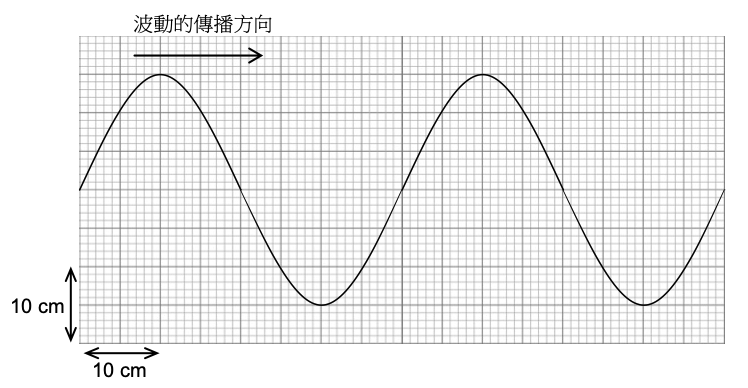
\includegraphics[width=.6\textwidth]{./img/ch1prob_2024-05-13-12-39-20.png}\par}
    \begin{parts}
        \part \begin{subparts}
            \subpart 這是橫波還是縱波?\zh{1}
            \subpart 粒子的振動和波動的傳播方向有甚麼關係?\zh{1}
        \end{subparts}
        \part 找出波動的
        \begin{subparts}
            \subpart 振幅。\zh{1}
            \subpart 波長。\zh{1}
            \subpart 週期。\zh{2}
            \subpart 速率。\zh{2}
        \end{subparts}
        \part 如果彈簧拉得更長,然後以相同的頻率振動,波動的速率、波長和週期會怎樣改變?\zh{3}
    \end{parts}

}{
    \sol
    \par{\par\centering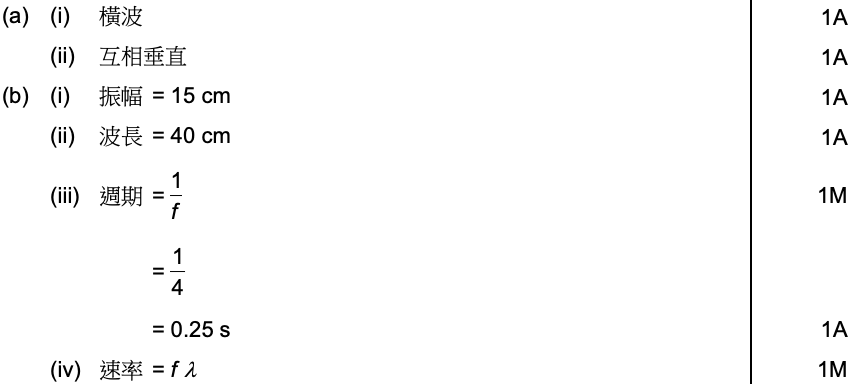
\includegraphics[width=\textwidth]{./img/ch1prob_2024-05-13-12-45-26.png}\par}
    \par{\par\centering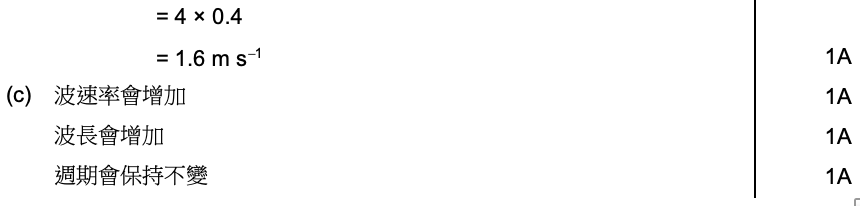
\includegraphics[width=\textwidth]{./img/ch1_earlyclass_wave_lq_2024-05-13-13-01-04.png}\par}
}

\newprob{1715576539}
{
    一列波沿繩子從左到右傳播。下圖顯示繩子在某時刻的形狀。
    \par{\par\centering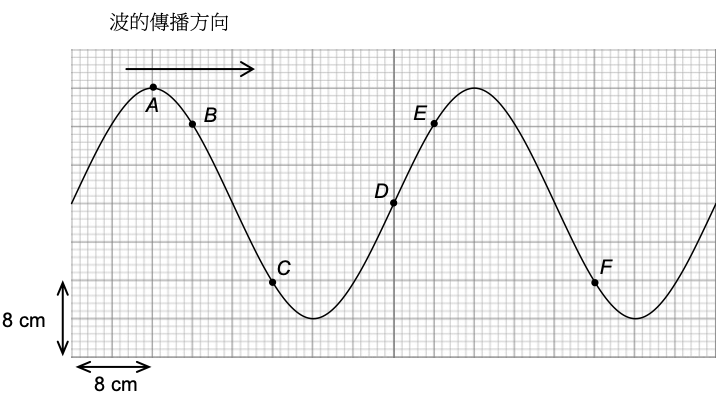
\includegraphics[width=.6\textwidth]{./img/ch1_earlyclass_wave_lq_2024-05-13-13-02-42.png}\par}
    \begin{parts}
        \part 這是橫波還是縱波?指出粒子振動方向和波動傳播方向的關係。\zh{2}
        \part \begin{subparts}
            \subpart 求波動的波長。\zh{1}
            \subpart 求波動的振幅。\zh{1}
        \end{subparts}
        \part \begin{subparts}
            \subpart 指出一對振動同相的粒子。\zh{1}
            \subpart 指出一對振動異相的粒子。\zh{1}
            \subpart 指出一對振動反相的粒子。\zh{1}
        \end{subparts}
        \part \begin{subparts}
            \subpart 指出一個向上移動的粒子。\zh{1}
            \subpart 指出一個向下移動的粒子。\zh{1}
            \subpart 指出一個瞬時靜止的粒子。\zh{1}
        \end{subparts}
    \end{parts}
}{
    \sol
    \par{\par\centering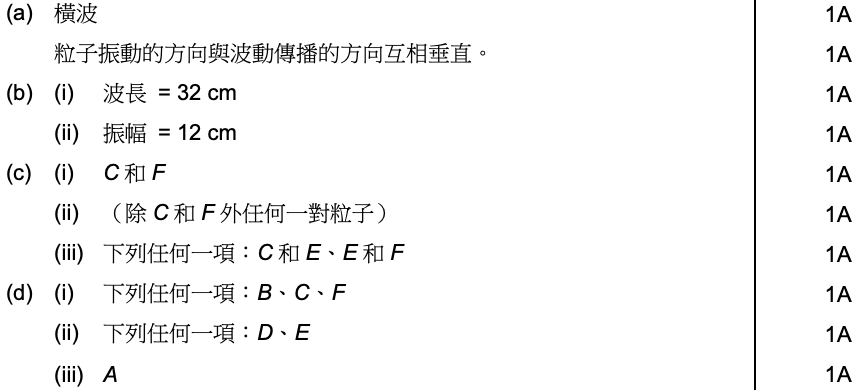
\includegraphics[width=\textwidth]{./img/ch1_earlyclass_wave_lq_2024-05-13-13-04-24.png}\par}
}

\newprob{1715576673}
{
    一列橫波在繩子中傳播。下圖顯示$t = 0$時繩子的波形。
    \par{\par\centering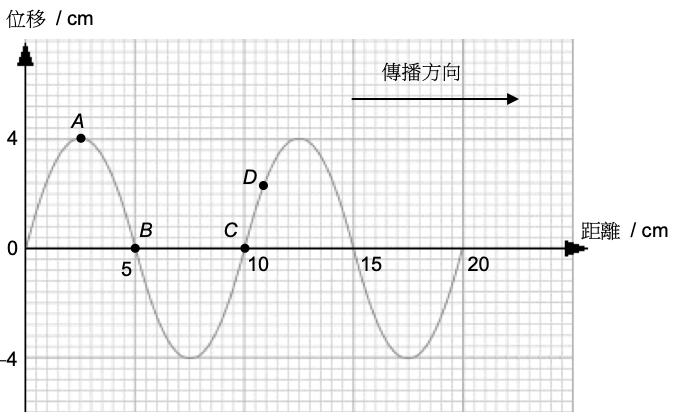
\includegraphics[width=.6\textwidth]{./img/ch1_earlyclass_wave_lq_2024-05-13-13-04-49.png}\par}
    \begin{parts}
        \part \begin{subparts}
            \subpart 指出橫波的定義。\zh{1}
            \subpart 舉出另一個橫波的例子。\zh{1}
        \end{subparts}
        \part \begin{subparts}
            \subpart 指出波動的振幅。\zh{1}
            \subpart 指出波動的波長。\zh{1}
        \end{subparts}
        \part 如果粒子$B$在2 s內完成5個振動週期,
        \begin{subparts}
            \subpart 求波動的頻率。\zh{1}
            \subpart 求波動的速率。\zh{2}
        \end{subparts}
        \part 考慮圖示的一刻,對以下各項舉出一個例子。
        \begin{subparts}
            \subpart 瞬時靜止的粒子\zh{1}
            \subpart 向上移動的粒子\zh{1}
            \subpart 向下移動的粒子\zh{1}
        \end{subparts}
        \part 如果波動的週期是0.4 s,草繪粒子A從t = 0 s到$t = 0.4$ s的位移—時間關係線圖。\zh{2}
    \end{parts}

}{
    \sol\par{\par\centering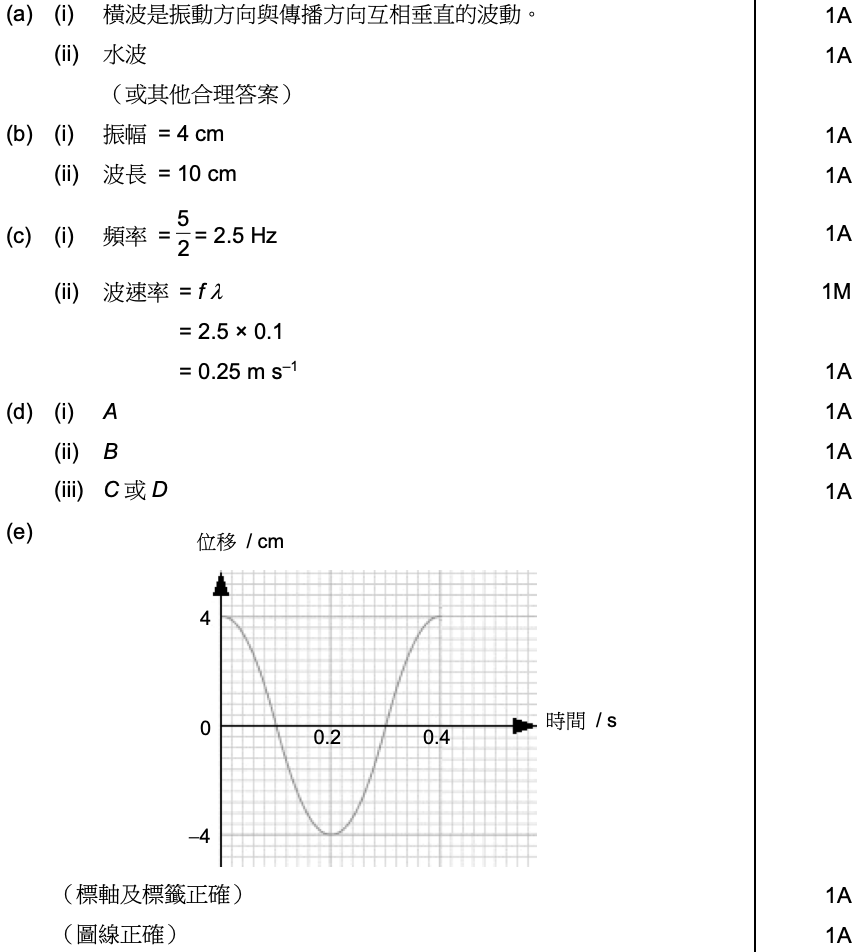
\includegraphics[width=\textwidth]{./img/ch1_earlyclass_wave_lq_2024-05-13-13-07-50.png}\par}
}

\newprob{1715576875}
{
    學生將軟彈簧放在地上並把一端固定,然後抖動另一端,產生橫波。下圖顯示彈簧上一個粒子$P$的位移—時間關係線圖。
    \par{\par\centering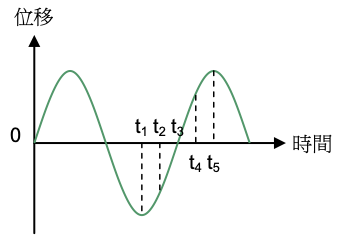
\includegraphics[width=.4\textwidth]{./img/ch1_earlyclass_wave_lq_2024-05-13-13-08-15.png}\par}
    \begin{parts}
        \part 寫出橫波的定義。\zh{1}
        \part 描述位移—時間關係線圖和位移—距離關係線圖的分別。\zh{2}
        \part 從$t_1$到$t_5$,粒子$P$分別在甚麼時候到達最大和最小速率?\zh{2}
        \part 提議怎樣量度彈簧中波的速率。\zh{3}
        \part 指出兩個影響波速率的因素。\zh{2}
    \end{parts}
    \dlines{1}\clearpage\dlines{1}

}{
    \sol\par{\par\centering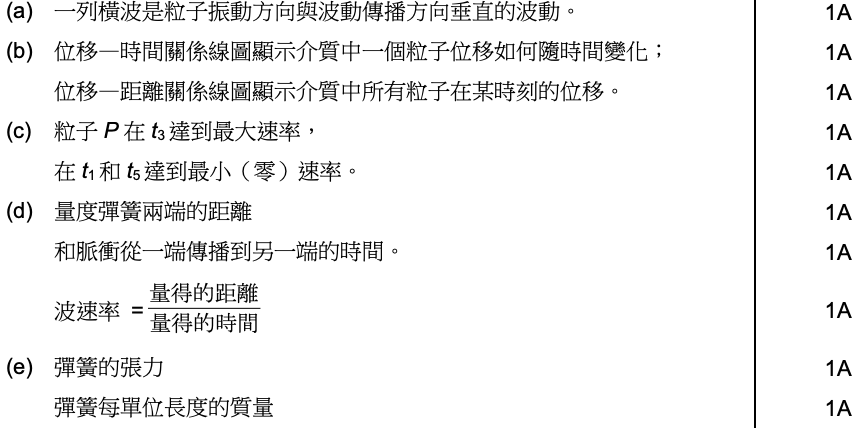
\includegraphics[width=\textwidth]{./img/ch1_earlyclass_wave_lq_2024-05-13-13-10-00.png}\par}
}

\newprob{1715577010}
{
    頻率為2 Hz的橫波沿繩子向右傳播,圖a顯示$t$ = 0時的波形,兩個相鄰波峯之間的距離是4 cm。波峯和波谷之間的垂直距離是6 cm。
    \par{\par\centering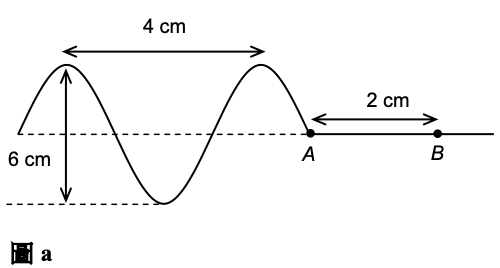
\includegraphics[width=.45\textwidth]{./img/ch1_earlyclass_wave_lq_2024-05-13-13-10-51.png}\par}
    \begin{parts}
        \part 找出波動的 \begin{subparts}
            \subpart 振幅。\zh{1}
            \subpart 週期。\zh{2}
            \subpart 速率。\zh{2}
        \end{subparts}
        \part $A$和$B$是繩子上兩個相距2 cm的粒子。
        \begin{subparts}
            \subpart 在圖b中草繪粒子$A$從$t$ = 0到$t$ = 1 s的位移—時間關係線圖。\zh{1}
            \par{\par\centering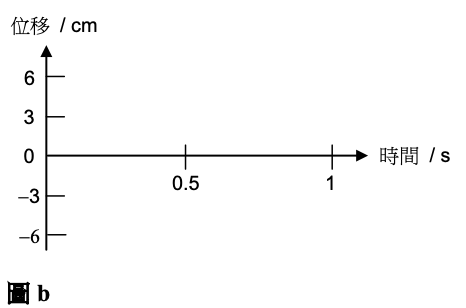
\includegraphics[width=.45\textwidth]{./img/ch1_earlyclass_wave_lq_2024-05-13-13-12-14.png}\par}
            \subpart 在圖c中草繪粒子$B$從$t$ = 0到$t$ = 1 s的位移—時間關係線圖。\zh{2}
            \par{\par\centering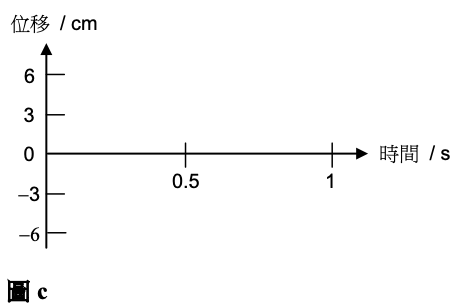
\includegraphics[width=.45\textwidth]{./img/ch1_earlyclass_wave_lq_2024-05-13-13-13-11.png}\par}
        \end{subparts}
        \part 粒子$A$和$B$的相位關係是甚麼?
    \end{parts}
}{
    {\par\centering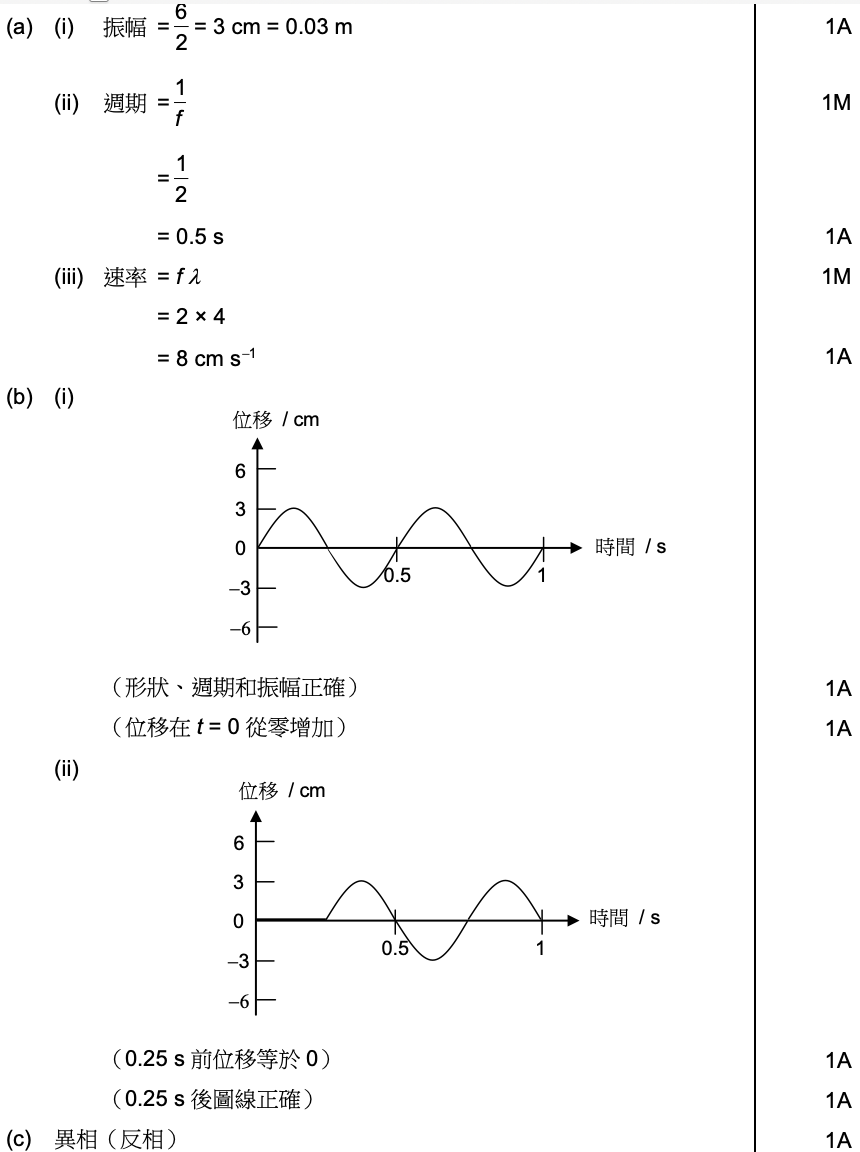
\includegraphics[width=\textwidth]{./img/ch1_earlyclass_wave_lq_2024-05-13-13-13-55.png}\par}
}


\newprob{1715577543}
{
    以下顯示行波上某粒子在$t$ = 0和$t$ = 0.3 s時的位移—距離關係線圖。
    \par{\par\centering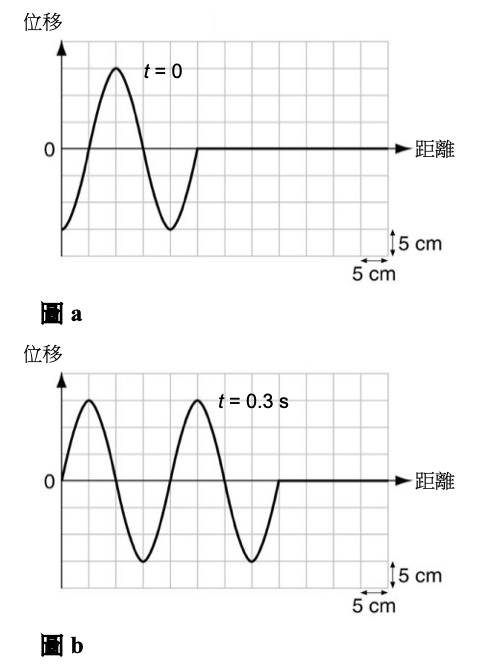
\includegraphics[width=.45\textwidth]{./img/ch1_earlyclass_wave_lq_2024-05-13-13-21-09.png}\par}
    % \par{\par\centering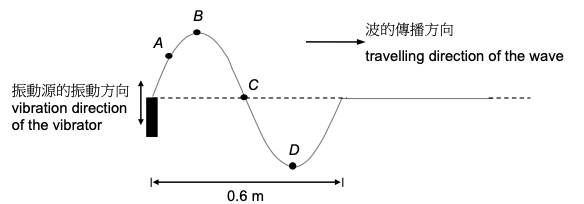
\includegraphics[width=.5\textwidth]{./img/ch1_weekend_wave_lq_2024-05-16-14-20-13.png}\par}
    \begin{parts}
        \part 找出行波的以下特性:
        \begin{subparts}
            \subpart 振幅\zh{1}
            \subpart 波長\zh{1}
            \subpart 速率\zh{2}
            \subpart 頻率\zh{2}
            \subpart 週期\zh{2}
        \end{subparts}
        \part 在圖b上繪畫波在t = 0.5 s時的位移—距離關係線圖。\zh{2}
    \end{parts}
}{
    \sol\par{\par\centering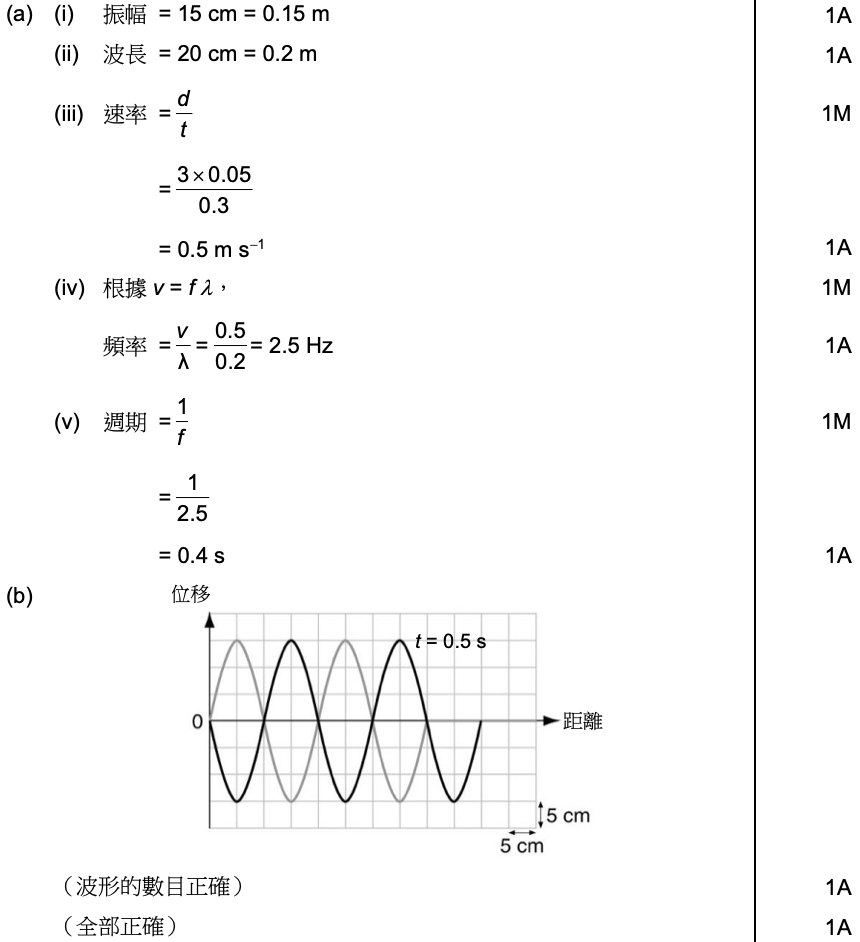
\includegraphics[width=\textwidth]{./img/ch1_earlyclass_wave_lq_2024-05-13-13-22-35.png}\par}
}

\newprob{1715577939}
{
    將橫波模型(圖a)安裝在高映機上,讓模型轉動,屏幕上便會出現一列向右傳播的橫波。假設某粒子在5秒內「上下振動」了10次。
    \par{\par\centering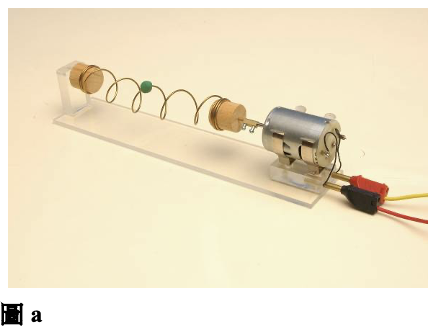
\includegraphics[width=.4\textwidth]{./img/ch1_earlyclass_wave_lq_2024-05-13-13-25-56.png}\par}
    \begin{parts}
        \part 橫波是甚麼?\zh{1}
        \part 圖b顯示「波」在t = 0時的位移—距離關係線圖。
        \par{\par\centering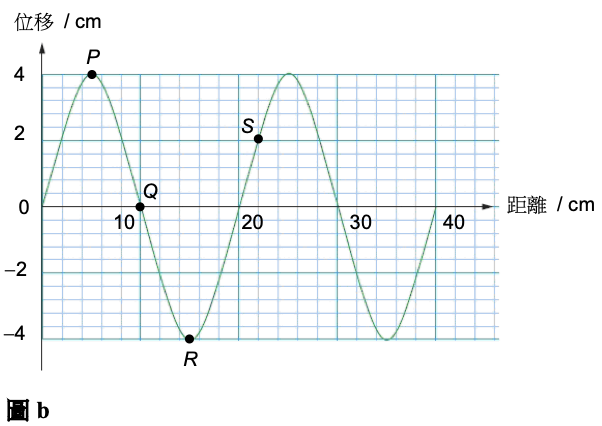
\includegraphics[width=.45\textwidth]{./img/ch1_earlyclass_wave_lq_2024-05-13-13-26-34.png}\par}
        \begin{subparts}
            \subpart 求「波」的振幅。\zh{1}
            \subpart 求「波」的波長。\zh{1}
        \end{subparts}
        \part 描述粒子$P$、$Q$、$R$和$S$在$t$ = 0時的運動。\zh{4}
        \part
        \begin{subparts}
            \subpart 求「波」的速率。\zh{2}
            \subpart 求「波」傳播80 cm所需的時間。\zh{2}
        \end{subparts}
        \part 草繪粒子Q從$t$ = 0到$t$ = 0.5 s的位移—時間關係線圖。\zh{2}
        \part 如果「波」的頻率增加,它的波長和波速率會怎樣改變?這與在彈簧上傳播的真實橫波有甚麼不同?\zh{2}
    \end{parts}
}{
    \sol\par{\par\centering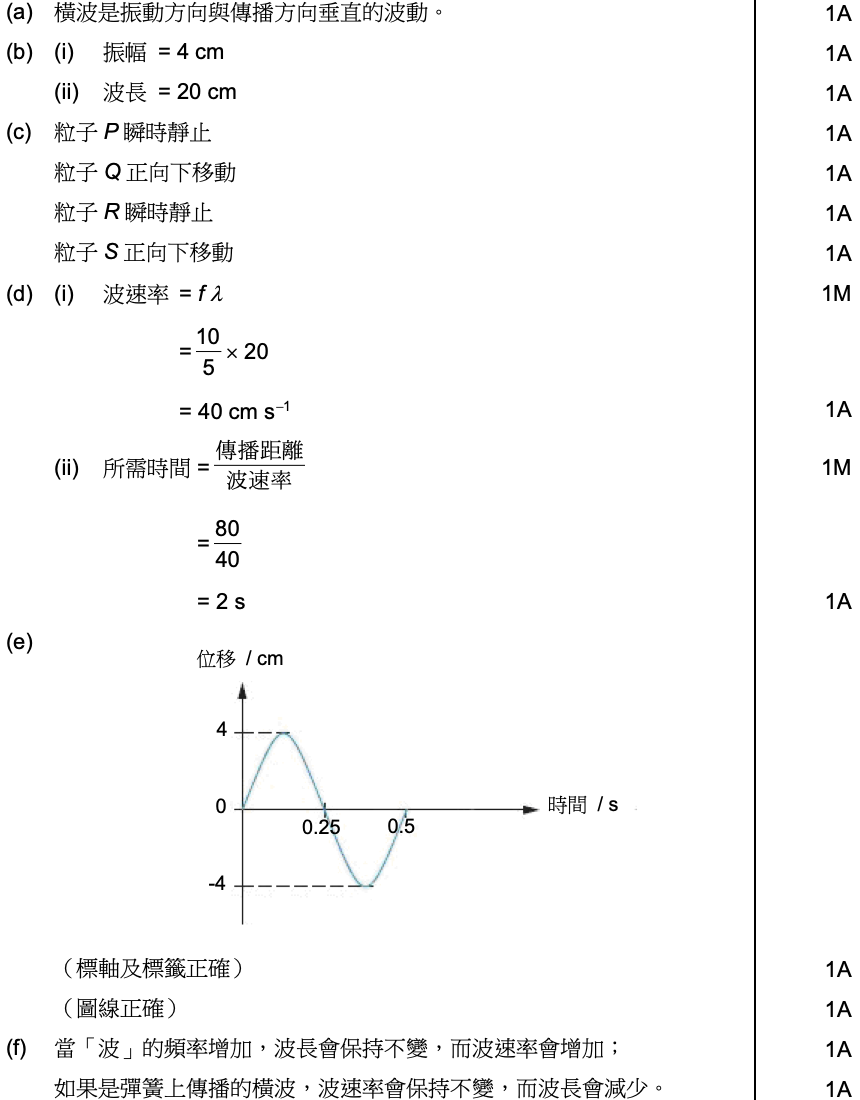
\includegraphics[width=\textwidth]{./img/ch1_earlyclass_wave_lq_2024-05-13-13-29-05.png}\par}
}

\newprob{1715588669}
{
    下圖顯示縱波的粒子在時間$t_1$的位置和平衡位置。
    \\The following figure shows the positions of particles on a travelling longitudinal wave at time $t_1$ and their equilibrium positions.
    % \par{\par\centering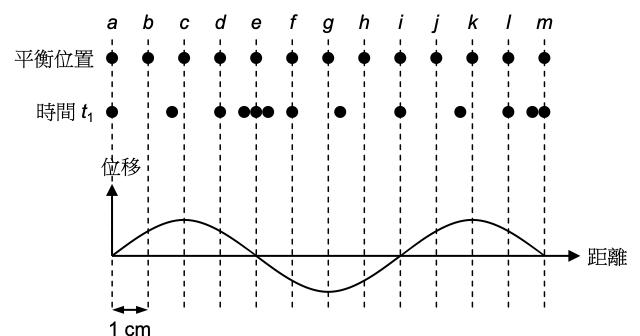
\includegraphics[width=.6\textwidth]{./img/ch1_earlyclass_wave_lq_2024-05-13-16-24-47.png}\par}
    \par{\par\centering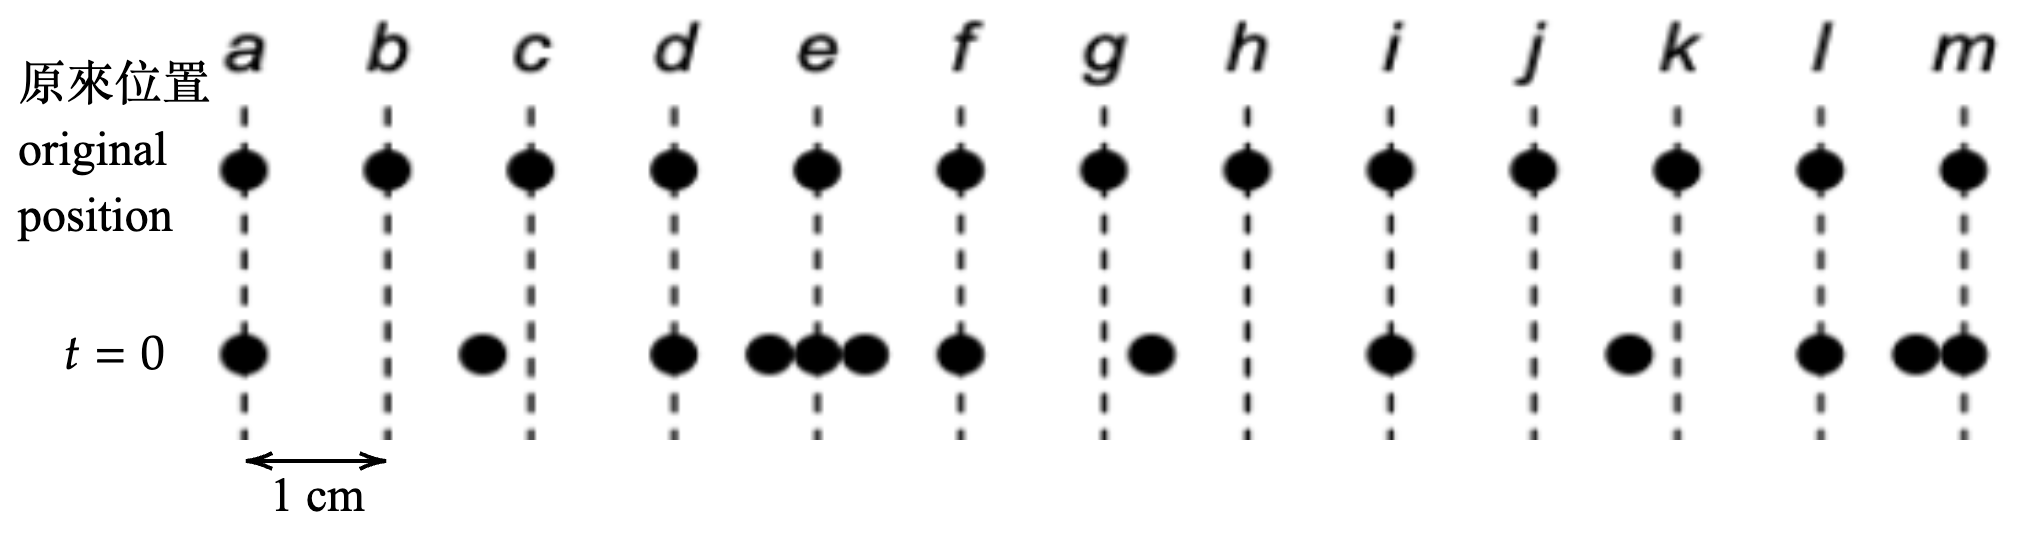
\includegraphics[width=.7\textwidth]{./img/ch1b_weekend_wave_lq_2024-05-24-16-00-47.png}\par}
    \begin{parts}
        \part 在某時間位移為零的粒子有什麼特性?\\What can you say about the particles having zero displacement at a certain time?\zh{2}
        \part 哪些粒子的振動有以下關係?各舉出一對粒子作例子。\\State one pair of particles in the figure that are\zh{1}
        \begin{subparts}
            \subpart 同相 in-phase\zh{1}
            \subpart 異相 anti-phase\zh{1}
            \subpart 反相 out of phase\zh{1}
        \end{subparts}
        \part \begin{subparts}
            \subpart 寫出波的波長。\\Write down the wavelength of the wave.\zh{1}
            \subpart 寫出波的振幅。\\Write down the amplitue of the wave.\zh{1}
        \end{subparts}
        \part 波動的頻率是3 Hz。求\\The frequency of wave is 3 Hz, find
        \begin{subparts}
            \subpart 振動的週期。\\the period.\zh{2}
            \subpart 波動的速率。\\speed of wave.\zh{2}
        \end{subparts}
    \end{parts}
    \dlines{1}\clearpage\dlines{1}\clearpage
}{
    \sol\par{\par\centering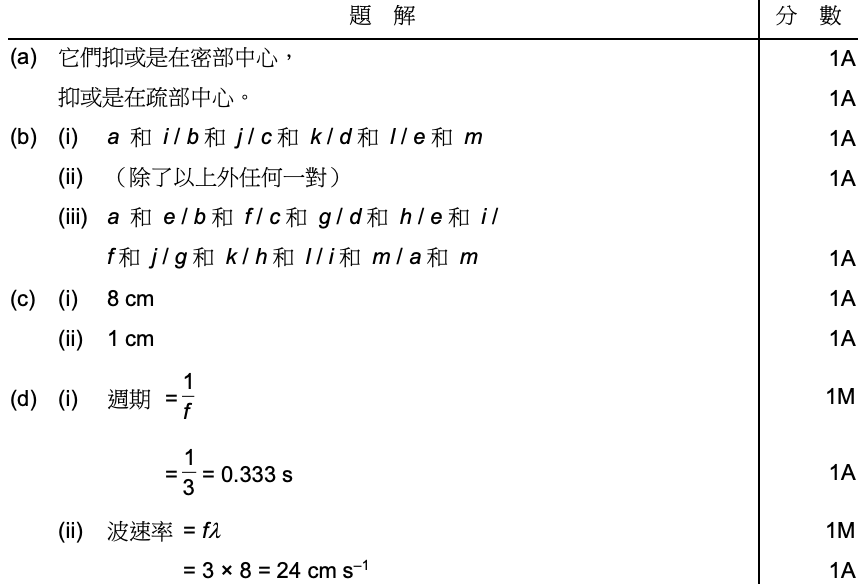
\includegraphics[width=\textwidth]{./img/ch1_earlyclass_wave_lq_2024-05-13-16-26-53.png}\par}

}

\newprob{1715588844}
{
    一塊膠泥貼在軟彈簧上,而軟彈簧從左邊持續推拉,使波動產生。
    \par{\par\centering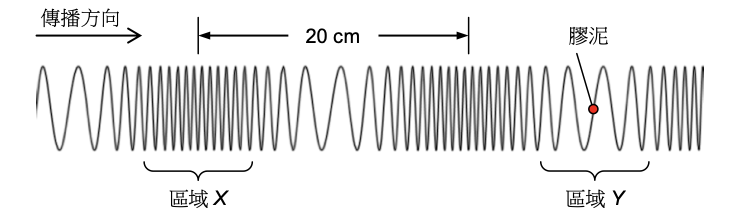
\includegraphics[width=.66\textwidth]{./img/ch1_earlyclass_wave_lq_2024-05-13-16-27-33.png}\par}
    \begin{parts}
        \part 指出 \begin{subparts}
            \subpart 所產生波動的種類。\zh{1}
            \subpart 區域X和Y的名字。\zh{2}
        \end{subparts}
        \part 指出膠泥在圖示一刻的運動方向。\zh{1}
        \part
        \begin{subparts}
            \subpart 指出波動的波長。\zh{1}
            \subpart 計算區域X和Y中心之間的距離。\zh{2}
        \end{subparts}
        \part \begin{subparts}
            \subpart 波動的頻率和膠泥振動的頻率有甚麼關係?\zh{1}
            \subpart 如果膠泥振動的頻率是0.5 Hz,求波的速率。\zh{2}
        \end{subparts}
    \end{parts}

}{
    \sol\par{\par\centering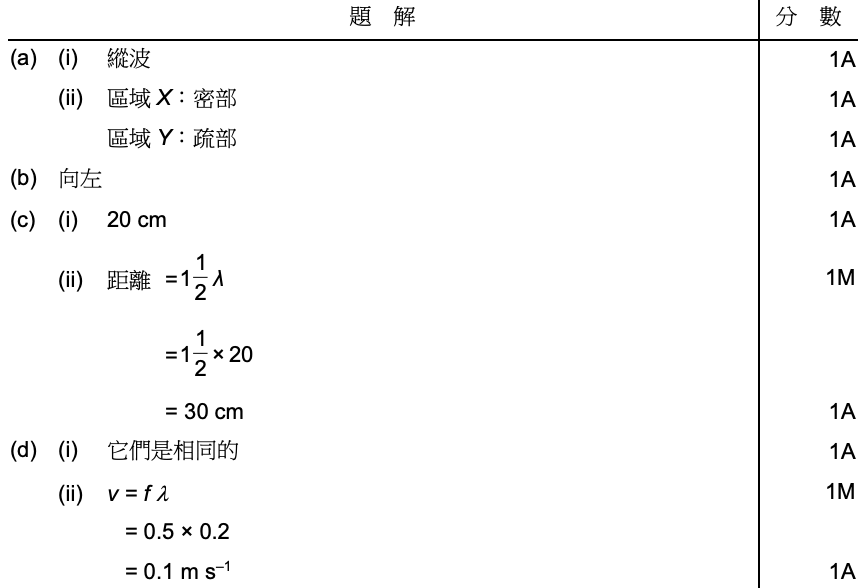
\includegraphics[width=\textwidth]{./img/ch1_earlyclass_wave_lq_2024-05-13-16-29-35.png}\par}
}

\newprob{1715601249}
{
    % my ex 1
    如圖所示,一列縱波從左至右以 \qty{0.3}{m.s^{-1}}的速率傳播,通過質點$A$至$M$,在$t=\qty{0}{s}$的情況。取向右的位移為正。\\As shown in the diagram, a longitudinal wave propagates from left to right with a speed of \vel{0.3}. It passes through points $A$ to $M$ at time $t = 0$. Take rightward direction as positive.
    \begin{figure}[h!]
        \centering
        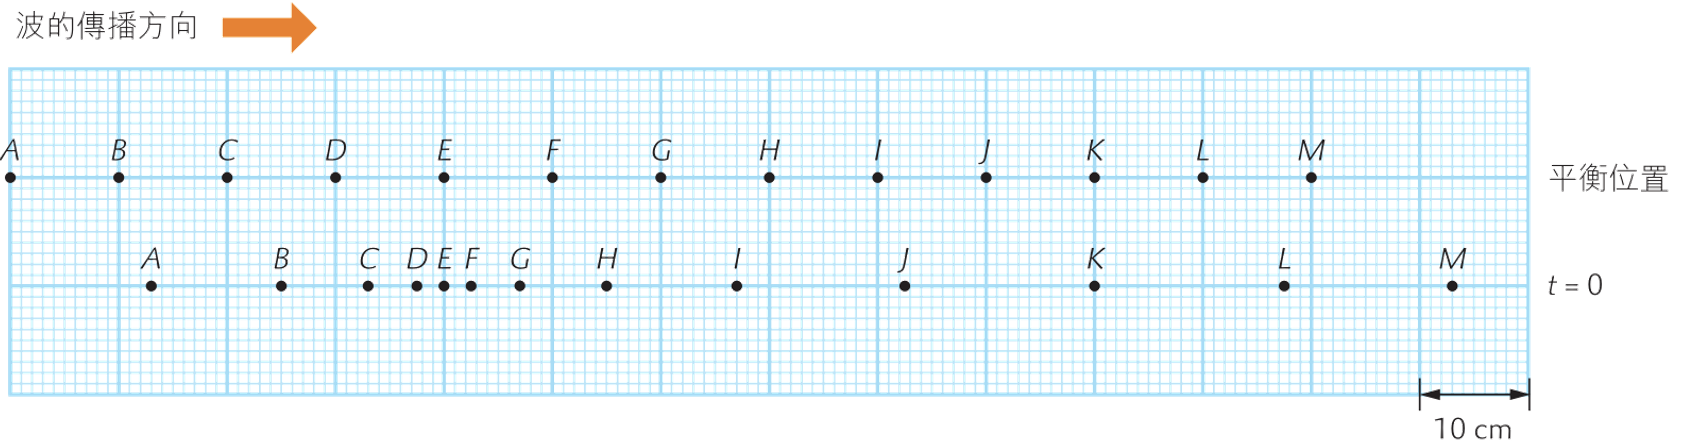
\includegraphics[width=\textwidth]{assets/da6d903d.png}
    \end{figure}
    \begin{parts}
        \part
        求波的週期,並草繪質點$B$、$E$、$H$ 和 $K$的$s$-$t$線圖。\\Find the period of wave, and sketch the displacement-time ($s$-$t$) graphs of $B$, $E$, $H$ and $K$.\par\zh{4}
        \begin{solutionbox}{\stretch{1}}

        \end{solutionbox}
        \clearpage
        \part
        如果這個縱波是從右至左以 \qty{0.6}{m.s^{-1}}的速率傳播,波長不變。求波的週期,並草繪質點$B$、$E$、$H$、$K$的$s$-$t$線圖。\\If this wave propagates from right to left at a velocity of \vel{0.6} without changing its wavelength, calculate the period of the wave and sketch the displacement-time ($s$-$t$) diagram for particles $B$, $E$, $H$, and $K$.\zh{4}
        \par{\par\centering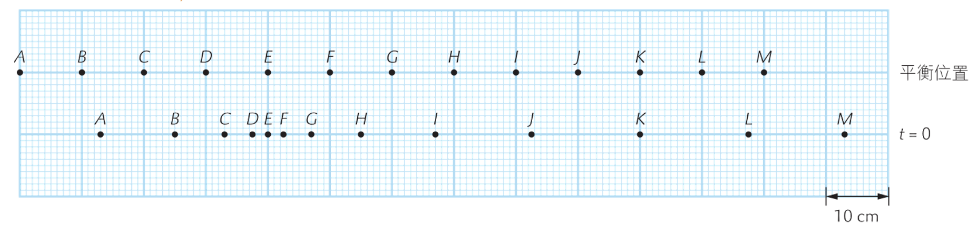
\includegraphics[width=\textwidth]{./img/ch1_earlyclass_wave_lq_2024-05-13-19-59-00.png}\par}
        \begin{solutionbox}{\stretch{1}}
        \end{solutionbox}
    \end{parts}
}{
    % 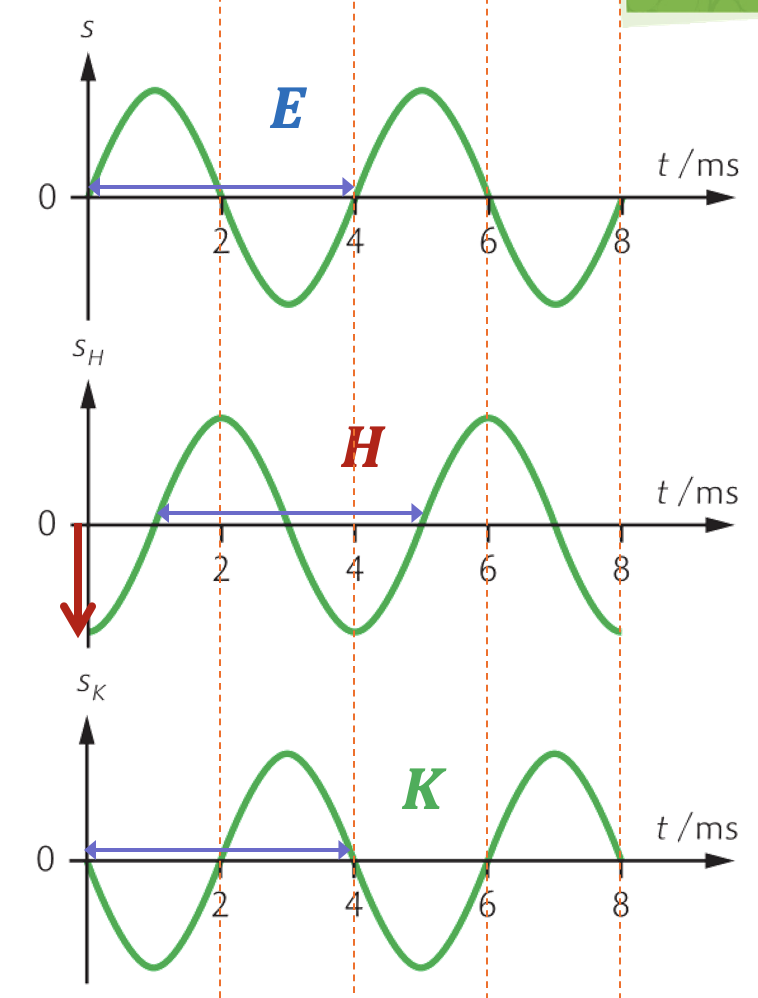
\includegraphics[width=0.5\textwidth]{assets/1f86230b.png}
    \sol
    \begin{enumerate}
        \item
              \topalign{\par\centering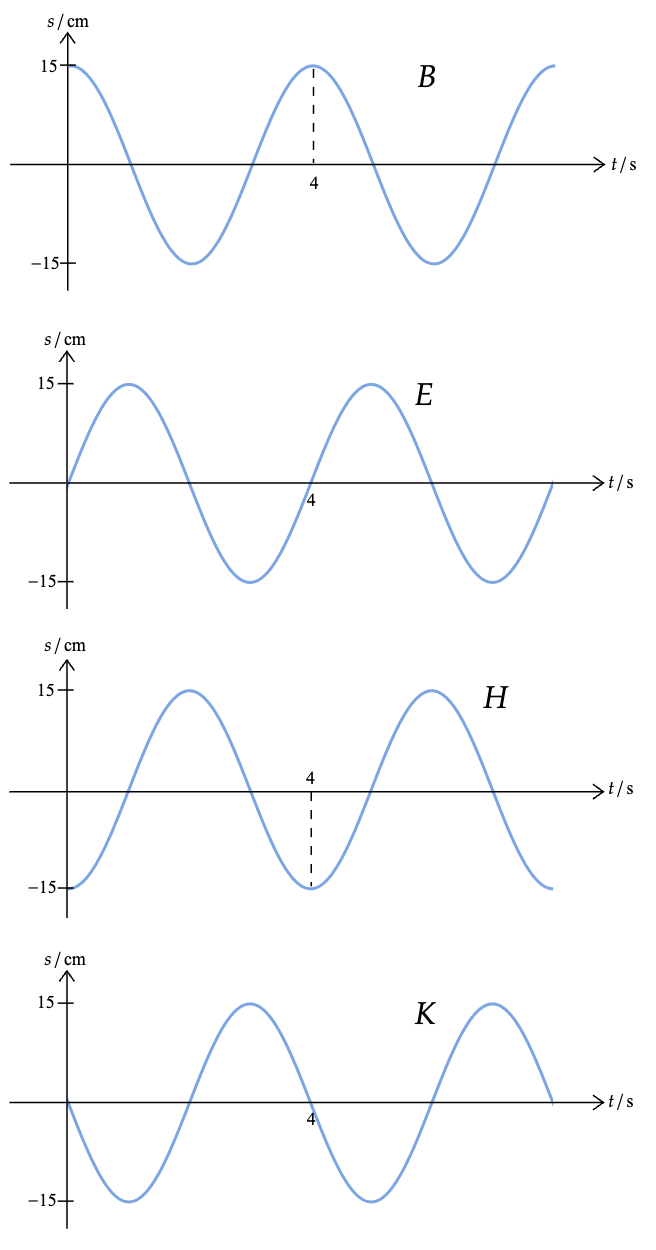
\includegraphics[width=.6\textwidth]{./img/ch1_earlyclass_wave_lq_2024-05-13-20-21-07.png}\par}
        \item
              \topalign{\par\centering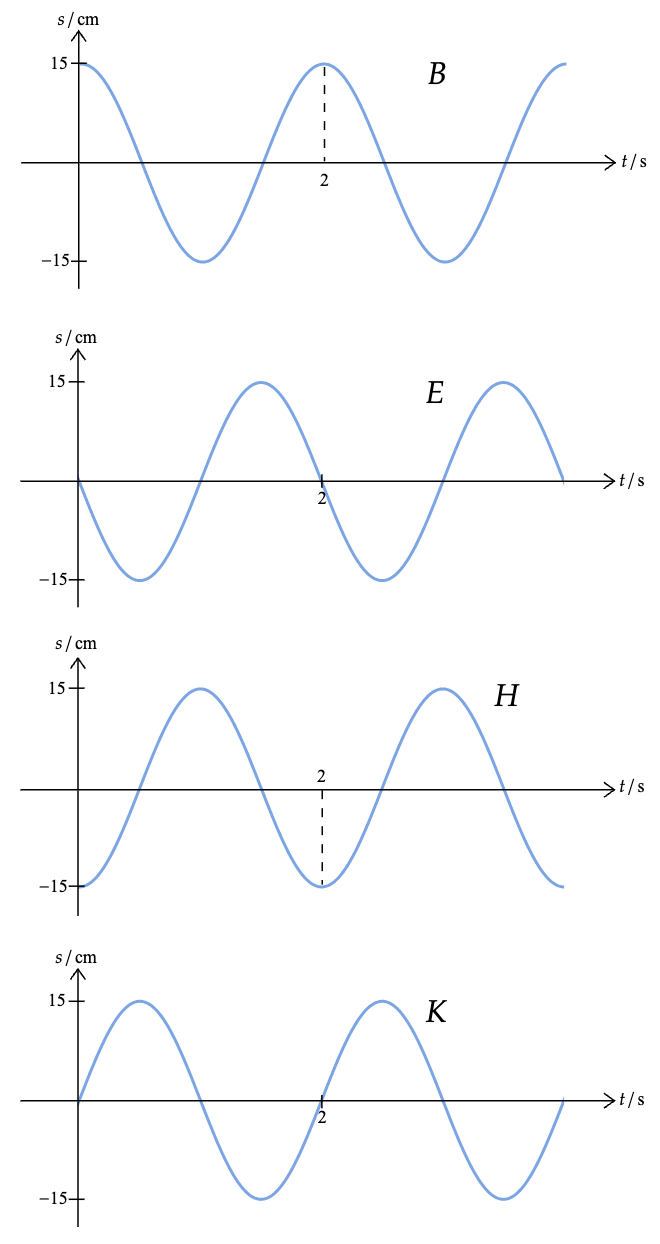
\includegraphics[width=.6\textwidth]{./img/ch1_earlyclass_wave_lq_2024-05-13-20-25-03.png}\par}
    \end{enumerate}
    % \par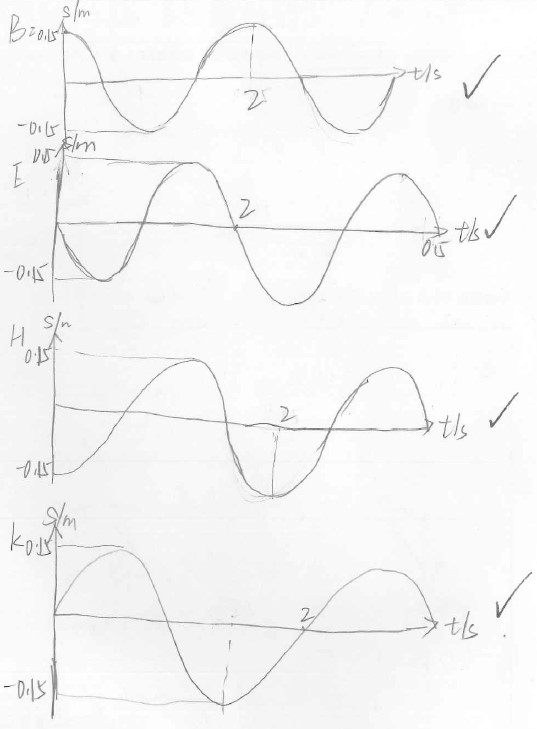
\includegraphics[width=0.8\linewidth]{assets/image.png}
}